\documentclass[]{beamer}
% \documentclass[handout]{beamer}
\usepackage[utf8]{inputenc}
% \usepackage{ulem}

\long\def\ignore#1{}

\newcommand{\Tanger}{{\sc Tanger}~}
\newcommand{\Siege}{{\em Siege}~}
\newcommand{\ManToHtml}{{\em man2html}~}
\newcommand{\obj}{{\tt obj}~}

\mode<presentation>
{
  \usetheme{Warsaw}
  % or ...
  %\usetheme{Darmstadt}
  %\setbeamertemplate{navigation symbols}{}

  \setbeamercovered{transparent}
  % or whatever (possibly just delete it)
}

\usepackage[english]{babel}

\pgfdeclareimage[height=0.5cm]{technion-logo}{Technion_-_Israel_Institute_of_Technology.pdf}
\pgfdeclareimage[height=1cm]{technion-logo-large}{Technion_-_Israel_Institute_of_Technology.pdf}

\title{Transactifying Apache's Cache Module}
\author[Haggai Eran, Ohad Lutzky, Zvika Guz, Idit Keidar]
{H.~Eran \and O.~Lutzky \and Z.~Guz \and I.~Keidar}
\institute
{
    Department of Electrical Engineering\\
    Technion -- Israel Institute of Technology
\and
    \pgfuseimage{technion-logo-large}
}
\date[SYSTOR'09]
{SYSTOR 2009 -- The Israeli Experimental Systems Conference}



\begin{document}

\begin{frame}
    \titlepage
\end{frame}

\logo{\pgfuseimage{technion-logo}}

\begin{frame}{Outline}
  \tableofcontents
  % You might wish to add the option [pausesections]
\end{frame}

\section{Introduction}
%\subsection{}

\begin{frame}{Transactifying Apache's Cache Module}
\begin{columns}[T]
\begin{column}{2cm}
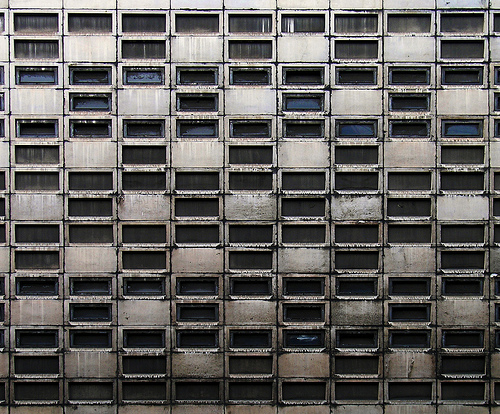
\includegraphics[width=\textwidth]{grid.jpg}
\end{column}
\begin{column}{8cm}
The shift to multicore machines challenges software developers to exploit
parallelism. Transactional Memory is one approach to make this easier.
\end{column}
\end{columns}
\pause

    \vspace{6pt} Our Goals:
    \begin{itemize}
        \item Transactifying a large-scale legacy application.
        \note{Experimenting and learning about the transactifycation process}
        \item Creating a performance evaluation method for STM systems.
    \end{itemize}    
\end{frame}

\begin{frame}{Why Apache?}
\begin{columns}[T]
\begin{column}{5cm}
\begin{itemize}
\item Large-scale
\item Popular
\item Already parallel
\end{itemize}
\end{column}
\begin{column}{5cm}

\includegraphics[width=\textwidth]{../apache_feather.png}
\end{column}
\end{columns}
\vspace{10pt}
\pause
And why Apache's Cache module?
\begin{itemize}
\item One of the points of interaction between Apache's worker threads.
\note{TODO: drawing...}
\item Well encapsulated.
\item Currently implemented using one big lock.
\note{Easily transactified.}
\end{itemize}
\end{frame}

\begin{frame}{Previous work}
\begin{columns}[T]
\begin{column}{8cm}
\begin{itemize}
\item Concurrent data structures \\ (e.g. red-black trees and skip lists.)
\item STMBench7 -- Measures operations on a more complex yet still artificial
      object graph. 
\item STAMP -- Standford Transactional Applications for Multi-Processing:\\
      A collection of transactified scientific algorithms.
\end{itemize}
\end{column}
\begin{column}{3cm}
\vspace{0.2cm}
  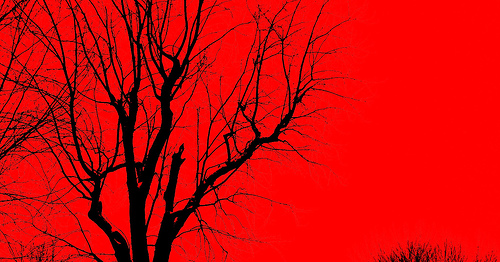
\includegraphics[width=\textwidth]{red-black-tree.jpg}
\vspace{0.2cm}
  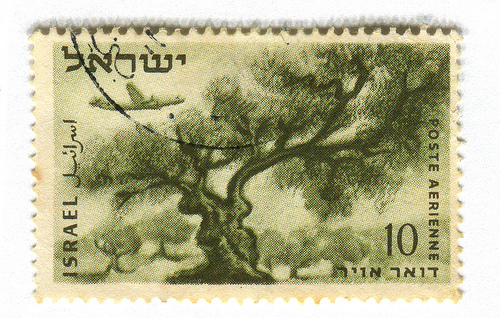
\includegraphics[width=\textwidth]{stamp.jpg}
\end{column}

\end{columns}
\end{frame}

\section{Transactification Process}
%\subsection{}

\begin{frame}{Which STM to use?}
    \begin{itemize}
        \item Library-based or \alert<2->{compiler-based}.
        \item<3-> {\Tanger}
            \begin{itemize}
                \item Open source
                \item LLVM compiler extension
                \item Supports tinySTM and other STM systems.
            \end{itemize}
        \item<3-> \alert<4->{Intel STM Compiler}
            \begin{itemize}
                \item Experimental version of Intel's ICC
                \item Proprietary STM system.
                \item Has published ABI for other STM systems.
            \end{itemize}
            \note{Chose Intel in spite of being proprietery because of
                  encapsulation difficulties with tanger.}
    \end{itemize}
\end{frame}

\begin{frame}{What to transactify}
\begin{enumerate}
\item Convert mutex critical sections into transactions.
\item Wrapping atomic instructions inside transactions.
\item Decorate functions with Intel's {\tt tm\_callable} attribute.
\end{enumerate}
\begin{center}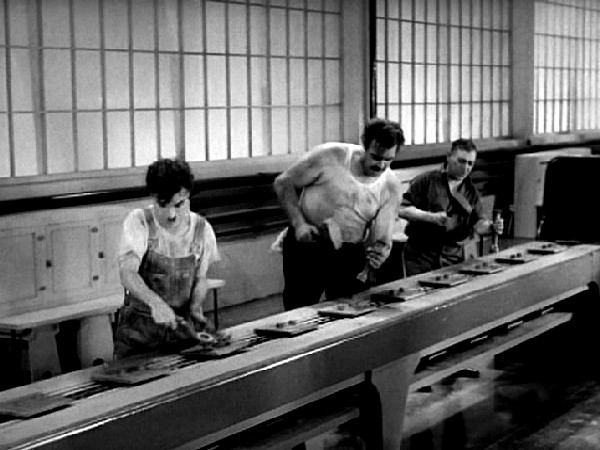
\includegraphics[height=4cm]{modern-times-assembly-line.jpg}\end{center}
\end{frame}

\begin{frame}{Defining Atomic Blocks}
Sometimes just converting a critical section in not optimal:
\begin{exampleblock}{Get an object from the cache}
\begin{enumerate}
\item<alert@1-2> \only<1>{Mutex lock}\only<2->{Begin transaction}
\item \obj $\leftarrow$ find key in cache
\item if \obj found
\begin{enumerate}
\item increment reference count on \obj
\item<alert@3> register \obj for reference count decrementation when done.
\end{enumerate}
\item<alert@1-2> \only<1>{Mutex unlock}\only<2->{End transaction}
\end{enumerate}
\end{exampleblock}
\end{frame}

\begin{frame}{Defining Atomic Blocks}
Suppose we know cleanup won't happen too soon.
\begin{exampleblock}{Get an object from the cache}
\begin{enumerate}
\item Begin transaction
\item \obj $\leftarrow$ find key in cache
\item if \obj found
\begin{enumerate}
\item increment reference count on \obj
\end{enumerate}
\item End transaction
\item<alert@1> if \obj found
\begin{enumerate}
\item register \obj for reference count decrementation when done.
\end{enumerate}
\end{enumerate}
\end{exampleblock}
\end{frame}
\begin{frame}{Commit Handlers}
\begin{columns}
\begin{column}{8cm}
\begin{itemize}
\item Pieces of code to be run on commit.
\item Together with abort handlers allow for more efficient transactions.
\item Can also be used in the shown scenario to clean up the code.
\end{itemize}
\end{column}
\begin{column}{3cm}
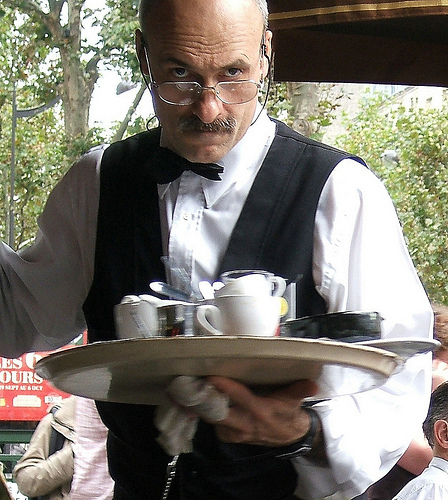
\includegraphics[width=\textwidth]{waiter.jpg}
\end{column}
\end{columns}
\end{frame}

\begin{frame}{Handler Closurs}
\begin{itemize}
\item Intel's commit handler syntax is: \begin{quote}
{\tt \_ITM\_addUserCommitAction(transaction, 
        commitFunction, 
        resumingTransactionId, 
        userArgument)
}
\end{quote}
\item Probably like any such construct in C.
\item In languages that support closures, the use of commit handlers for our
      purpose would be much cleaner.  
\end{itemize}
\end{frame}

\begin{frame}{Statistics and Profiling}
[TODO - a single line somewhere - not an entire slide.]
\end{frame}

\section{Results}
%\subsection{}
\begin{frame}{Evaluation}
\begin{description}
\item[Client] The \Siege HTTP load testing tool.
\item[Workload] The set of unix man-pages, served using the \ManToHtml CGI
                program. The program uncompressed the man-pages and rendered
                them to HTML.
\item[Distribution] Request files by Zipf distribution, whose $s$ parameter
determines the level of localilty in the requests.
\item[Setup] Two machines connected by Gigabit ethernet, each an 8-processors
SMP with quard core 2.3GHz AMD Opteron processors and 126GB of RAM.
\end{description}
\end{frame}

\begin{frame}{Results -- Requests per Second}
\framesubtitle{$s=0.1$}
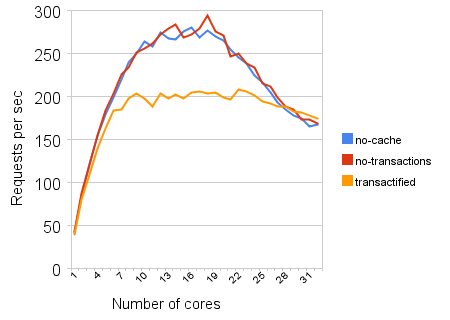
\includegraphics[width=\textwidth, trim=1cm 9.5cm 0 10.6cm]{../SYSTOR09/transaction-rate-client-server-0dot1.pdf}

Very \alert{low} locality. Cache not effective. STM penalty high.
\end{frame}

\begin{frame}{Results -- Requests per Second}
\framesubtitle{$s=1$}
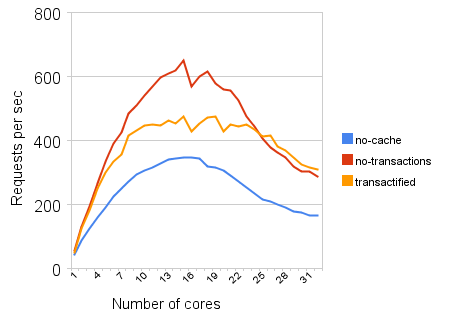
\includegraphics[width=\textwidth, trim=1cm 9.5cm 0 10.6cm]{../SYSTOR09/transaction-rate-client-server-1.pdf}

\alert{Medium} locality. Cache is an improvement. STM incurs penalty.
\end{frame}

\begin{frame}{Results -- Requests per Second}
\framesubtitle{$s=2$}
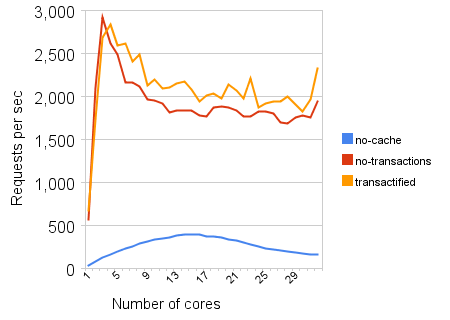
\includegraphics[width=\textwidth, trim=1cm 9.5cm 0 10.6cm]{../SYSTOR09/transaction-rate-client-server-2.pdf}

\alert{High} locality. Cache is vital. STM version works best.
\end{frame}

%TODO - Abort rate slides
\section{Summary}
%\subsection{}

\begin{frame}{Conclusion}
\begin{itemize}
\item Encapsulation is important.
\item Commit handlers might be useful not only for open transactions.
\item Real-world applications are challenging and important to work on.
\end{itemize}
\end{frame}

\begin{frame}{Questions?}
\begin{center}
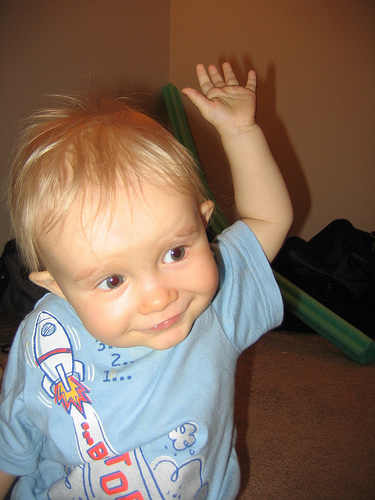
\includegraphics[height=5cm]{raisehand.jpg}
\end{center}
\end{frame}

\end{document}
